\documentclass[article]{memoir}

\usepackage[utf8]{inputenc}
\usepackage{babel}
\usepackage{stfloats}
\usepackage{microtype}
\usepackage{graphicx}
\usepackage{pdfpages}
\tolerance=1
\emergencystretch=\maxdimen
% \usepackage{tgtermes}
\usepackage{hyperref}
\usepackage{xcolor}
\hypersetup{
  colorlinks,
  linkcolor={red!50!black},
  citecolor={blue!50!black},
  urlcolor={blue!80!black},
  pdftitle={Grizzards Unerase Utility Manual},
  pdfsubject={Grizzards videogame for the Atari 2600},
  pdfauthor={Bruce-Robert Pocock}%,
  % pdfkeywords={Your PDF keywords}
}


\title{Grizzards Unerase Utility}
\author{Bruce-Robert Pocock}

\begin{document}

\chapter*{Grizzards Unerase Utility}

\section*{What is it?}

This utility has only one purpose:  If you have accidentally erased your
game  in progress  in  the  game \textit{Grizzards},  it  allows you  to
recover it.

\section*{Limitations}

This  utility must  be  used \textit{only}  immediately  after the  game
was erased. In particular, you must \textit{not} have started a new game
in the same ``slot'' yet.

This utility  only works with  the full version of  the game. It  is not
useful for the demo version.

\section*{Accessing The Utility}

In order to use this program, you  will need a utility cartridge such as
the Harmony (or Harmony Encore), Uno, or PlusCart.

First, make sure that your SaveKey, MemCard, or AtariVox is connected to
the right controller port on your Atari console.

For    the    Harmony    or     Uno    cartridge,    copy    the    file
\texttt{Grizzards.Unerase.NTSC.a26} (in North America, Brazil, Korea, or
Japan), \texttt{Grizzards.Unerase.PAL.a26}  (in Europe,  except France),
or \texttt{Grizzards.Unerase.SECAM.a26}  (in France, Russia,  or Africa)
to your SD  card. Start up your  Atari console with your  Harmony or Uno
cartridge and select the Unerase utility from the menu.

For the PlusCart, you can access the Unerase utility from the PlusStore.
Navigate  to the  Grizzards folder  in  the PlusStore  and download  the
Unerase image appropriate to your region.

\clearpage

\section*{How To Use}

The utility will display a screen like the below:

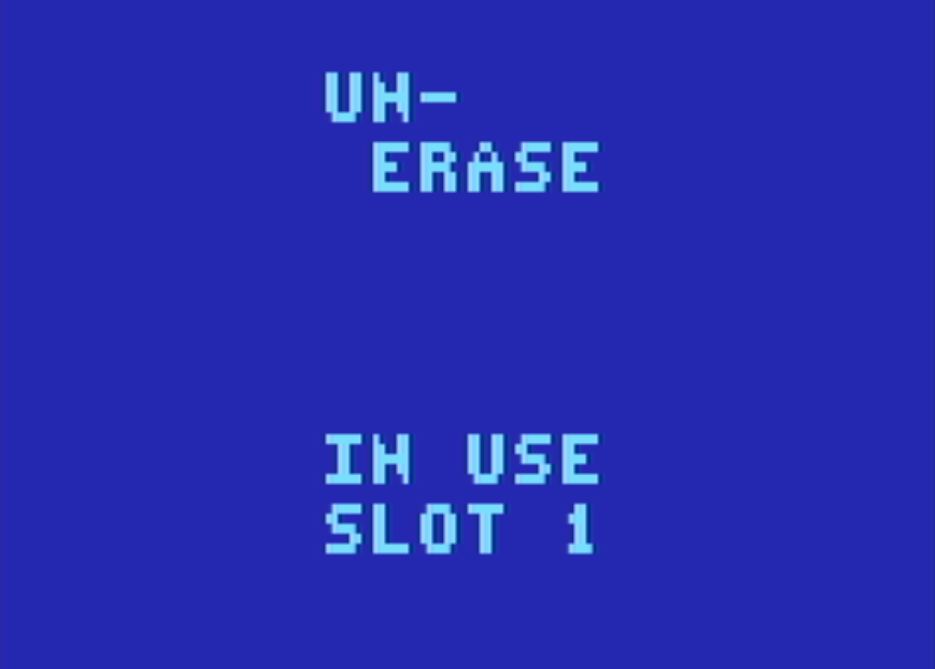
\includegraphics[width=\columnwidth]{../Manual/Unerase.png}

Press the \textbf{Game Select} switch to select a save game slot. As you
select each slot, you will see its current status:

\begin{itemize}
\item \texttt{IN USE} is a slot which has an active save game record.
\item \texttt{BLANK}  is a slot  which has not  been used, or  which has
  been erased too thoroughly to recover.
\item \texttt{ERASED} is a slot which  contains a save game record which
  has been erased, but can be recovered.
\end{itemize}

When you have selected a slot which contains an erased save game record,
you can  press the  \textbf{Game Reset} switch  to recover  that record.
If  successful,  the  indicator  will  change  from  \texttt{ERASED}  to
\texttt{IN USE}.

\section*{For Further Assistance}

If you need further assistance, check the \textit{Grizzards} web site at
\href{https://star-hope.org/games/Grizzards/}{https://\-star-hope.org/\-games/\-Grizzards/}
or eMail \href{mailto:support@star-hope.org}{support@star-hope.org}.

\vfill

Copyright \copyright 2021-2022 Bruce-Robert Pocock

\end{document}
